\documentclass[../main.tex]{subfiles}
\graphicspath{{\subfix{../diagrams/}}}


\begin{document}

\section{Privileged ISA}
RISC-V provides privilege architecture which includes privileged instructions as well as additional functionality required for running operating system and attaching external device.

\subsubsection{RISC-V Privileged Software Stack Terminology}
The RISC-V ISA defines a wide range of possible privileged software stacks.

\begin{figure}[h]
\centering
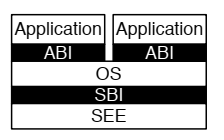
\includegraphics[width=5cm]{diagrams/risc_v_stack.png}
\caption{Conventional operating system}
\label{fig:software_stack}
\end{figure}

\noindent Since we targeted to run an operating system on our RISC-V core, we intended to use the following configuration shown in figure \ref{fig:software_stack} that can support multi-programmed execution of multiple applications. Each application communicates over an application binary interface (ABI) with the OS. RISC-V
operating systems interface with a supervisor execution environment (SEE), This environment consists of the supervisor-mode instructions and CSRs defined by the privileged ISA document. In this section we discuss the privileged ISA set by the RISC-V specification \cite{riscvpriv} and the selected set implemented in our processor.

\subsection{Privilege Levels and CSRs}
\subsubsection{Privilege Levels}
As described in the privileged ISA document, a RISC-V hardware thread (hart) is running at some privilege level encoded as a mode in one or more CSRs (control and status registers). There are three privilege levels defined as shown in table \ref{tab:modes}. These privilege levels are used to provide protection between different components of the software stack, and attempts to perform operations not permitted by the current privilege mode will cause an exception to be raised. These exceptions will normally cause traps into an underlying execution environment.\\
\newline
\noindent The machine level has the highest privileges and is the only mandatory privilege level for a RISC-V hardware platform, As this is the only mode that has unfettered access to the whole machine. But since we need to run OS we implemented the other two modes (S, U).

\begin{table}[h]
\begin{center}
\begin{tabular}{ |c|c|c|c| } 
\hline
Level & Encoding & Name & Abbreviation \\
\hline
\multirow 
0 & 00 & User/Application & U \\ 
1 & 01 & Supervisor & S \\ 
2 & 10 & Reserved &  \\ 
3 & 11 & Machine & M \\
\hline
\end{tabular}
\end{center}
\caption{RISC-V privilege levels.}
\label{tab:modes}
\end{table}

\subsubsection{Control and Status Registers (CSRs)}
Control and status registers (CSR) are register that store various information in CPU. RISC-V defines a separate address space of 4096 CSRs so we can have at most 4096 CSRs. RISC-V only allocates a part of address space so we can add custom CSRs in unused addresses. Also, not all CSRs are required on all implementations.\\By convention, the upper 4 bits of the CSR address (csr[11:8]) are used to encode the read and write accessibility of the CSRs according to privilege level as shown in Table 2.1. The top two bits (csr[11:10]) indicate whether the register is read/write (00, 01, or 10) or read-only (11). The next two bits (csr[9:8]) encode the lowest privilege level that can access the CSR.\\ 
\newline
\noindent In our micro-architecture we only implement the required CSRs for the the modes to support interrupt handling, exceptions, in addition to the timer interrupts registers. Also, we implemented four custom CSRs for the crypto-IP integration.
The implemented CSR registers are listed in tables \ref{tab:user_CSRs},  \ref{tab:super_CSRs}, \ref{tab:machine_CSRs}, and \ref{tab:CSRs2} with their addresses and names in our implementation.

\begin{table}[p]
\centering
\begin{tabular}{|c|c|p{3.5cm}| p{6.2cm}|} 
\hline
CSR address & Privilege & Name & Description \\
\hline
\multicolumn{4}{|c|}{User Trap Setup}\\
\hline
0x000 & URW & CSR\_USTATUS & User status register\\
0x004 & URW & CSR\_UIE & User interrupt-enable register\\
0x005 & URW & CSR\_UTVEC & User trap-handler base address\\
\hline
\multicolumn{4}{|c|}{User Trap Handling}\\
\hline
0x140 & URW & CSR\_USCRATCH & Scratch register for Supervisor trap handlers\\
0x041 & URW & CSR\_UEPC & Supervisor exception program counter\\
0x042 & URW & CSR\_UCAUSE & Supervisor trap cause\\
0x043 & URW & CSR\_UTVAL & Supervisor bad address or instruction\\
0x044 & URW & CSR\_UIP & Supervisor interrupt pending\\
\hline
\multicolumn{4}{|c|}{User Counter/Timers}\\
\hline
0xC00 & URW & CSR\_CYCLE & Cycle counter for RDCYCLE instruction\\
0xC01 & URW & CSR\_TIME & Timer for RDTIME instruction\\
0xC02 & URW & CSR\_INSTERT & counter for RDINSTRET instruction\\
0x8FF & URW & CSR\_UNECYCLE & User timer\\
\hline
\end{tabular}
\caption{Implemented user mode CSRs.}
\label{tab:user_CSRs}
\end{table}

\begin{table}[p]
\centering
%p{3cm} | p{2.8cm} | p{2.5cm} | p{1.5cm} | p{2.7cm} |
\begin{tabular}{|c|c|p{3.5cm}| p{6.2cm}|} 
\hline
CSR address & Privilege & Name & Description \\
\hline
\multicolumn{4}{|c|}{Supervisor Trap Setup}\\
\hline
0x100 & SRW & CSR\_SSTATUS & Supervisor status register\\
0x102 & SRW & CSR\_SEDELEG & Supervisor exception delegation register\\
0x103 & SRW & CSR\_SIDELEG & Supervisor interrupt delegation register\\
0x104 & SRW & CSR\_SIE & Supervisor interrupt-enable register\\
0x105 & SRW & CSR\_STVEC & Supervisor trap-handler base address\\
0x106 & SRW & CSR\_SCOUNTEREN & Supervisor counter enable\\
\hline
\multicolumn{4}{|c|}{Supervisor Trap Handling}\\
\hline
0x140 & SRW & CSR\_SSCRATCH & Scratch register for Supervisor trap handlers\\
0x141 & SRW & CSR\_SEPC & Supervisor exception program counter\\
0x142 & SRW & CSR\_SCAUSE & Supervisor trap cause\\
0x143 & SRW & CSR\_STVAL & Supervisor bad address or instruction\\
0x144 & SRW & CSR\_SIP & Supervisor interrupt pending\\
\hline
\end{tabular}
\caption{Implemented supervisor mode CSRs.}
\label{tab:super_CSRs}
\end{table}

\begin{table}[h]
\centering
%p{3cm} | p{2.8cm} | p{2.5cm} | p{1.5cm} | p{2.7cm} |
\begin{tabular}{|c|c|p{3.5cm}| p{6.2cm}|} 
\hline
CSR address & Privilege & Name & Description \\
\hline
\multicolumn{4}{|c|}{Machine Information Registers}\\
\hline
0xF11 & MRO & CSR\_MVENDORID & Vendor ID \\ 
0xF12 & MRO & CSR\_MARCHID & Architecture ID \\ 
0xF13 & MRO & CSR\_MIMPID &  Implementation ID\\ 
0xF14 & MRO & CSR\_MHARTID & Hardware thread ID\\
\hline
\multicolumn{4}{|c|}{Machine Trap Setup}\\
\hline
0x300 & MRW & CSR\_MSTATUS & Machine status register\\
0x301 & MRW & CSR\_MISA & ISA and extensions\\
0x302 & MRW & CSR\_MEDELEG & Machine exception delegation register\\
0x303 & MRW & CSR\_MIDELEG & Machine interrupt delegation register\\
0x304 & MRW & CSR\_MIE & Machine interrupt-enable register\\
0x305 & MRW & CSR\_MTVEC & Machine trap-handler base address\\
0x306 & MRW & CSR\_MCOUNTEREN & Machine counter enable\\
\hline
\multicolumn{4}{|c|}{Machine Trap Handling}\\
\hline
0x340 & MRW & CSR\_MSCRATCH & Scratch register for machine trap handlers\\
0x341 & MRW & CSR\_MEPC & Machine exception program counter\\
0x342 & MRW & CSR\_MCAUSE & Machine trap cause\\
0x343 & MRW & CSR\_MTVAL & Machine bad address or instruction\\
0x344 & MRW & CSR\_MIP & Machine interrupt pending\\
\hline
\multicolumn{4}{|c|}{Machine Counter/Timers}\\
\hline
0xB00 & MRW & CSR\_MCYCLE & Machine cycle counter\\
0xB02 & MRW & CSR\_MINSTRET & Machine instructions-retired counter\\
0xB80 & MRW & CSR\_MCYCLEH & Upper 32 bits of mcycle, RV32I only\\
0xB82 & MRW & CSR\_MCYCLEH & Upper 32 bits of minstret, RV32I only\\
\hline
\end{tabular}
\caption{Implemented machine mode CSRs.}
\label{tab:machine_CSRs}
\end{table}

\begin{table}[t!]
\centering
\begin{tabular}{ |c|c|p{3.5cm}| p{6.2cm}|} 
\hline
CSR address & Privilege & Name & Description \\
\hline
\multicolumn{4}{|c|}{Custom CSRs for the Encryption IP}\\
\hline
0x7C0 & MRW & CSR\_AES\_D0 & lowest 32 bits of data\\
0x7C1 & MRW & CSR\_AES\_D1 & data from 32:63\\
0x7C2 & MRW & CSR\_AES\_D2 & data from 64:95\\
0x7C3 & MRW & CSR\_AES\_D3 & highest 32 bits of data\\
0x7C4 & MRW & CSR\_AES\_key & key address\\
\hline
\end{tabular}
\caption{Implemented AES CSRs.}
\label{tab:CSRs2}
\end{table}

\subsection{“Zicsr”, Control and Status Register Instructions}
This extension defines the full set of CSR instructions that operate on the CSRs.\\
\newline
\noindent All CSR instructions atomically read-modify-write a single CSR, whose CSR specifier is encoded in the 12-bit csr field of the instruction held in bits 31–20. The immediate forms use a 5-bit zero-extended immediate encoded in the rs1 field as shown in figure \ref{fig:csr_inst}.

\begin{figure}[t]
\centering
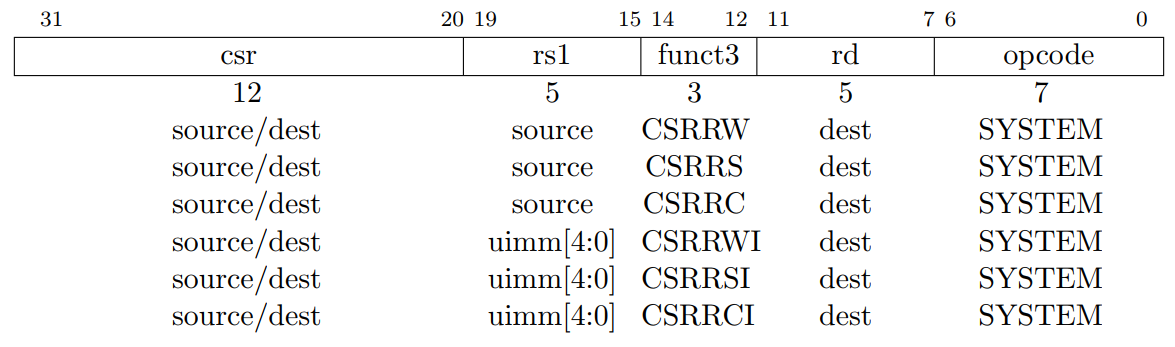
\includegraphics[width=15 cm]{diagrams/csr_inst.png}
\caption{CSR Instructions}
\label{fig:csr_inst}
\end{figure}

\noindent The CSRRW (Atomic Read/Write CSR) instruction atomically swaps values in the CSRs and integer registers. CSRRW reads the old value of the CSR, zero-extends the value to XLEN bits, then writes it to integer register rd. The initial value in rs1 is written to the CSR. If rd=x0, then the instruction shall not read the CSR and shall not cause any of the side effects that might occur on a CSR read.\\
\\The CSRRS (Atomic Read and Set Bits in CSR) instruction reads the value of the CSR, zero-extends the value to XLEN bits, and writes it to integer register rd. The initial value in integer register rs1 is treated as a bit mask that specifies bit positions to be set in the CSR. Any bit that is high in rs1 will cause the corresponding bit to be set in the CSR, if that CSR bit is writable. Other bits in the CSR are unaffected (though CSRs might have side effects when written).\\
\\The CSRRC (Atomic Read and Clear Bits in CSR) instruction reads the value of the CSR, zeroextends the value to XLEN bits, and writes it to integer register rd. The initial value in integer register rs1 is treated as a bit mask that specifies bit positions to be cleared in the CSR. Any bit that is high in rs1 will cause the corresponding bit to be cleared in the CSR, if that CSR bit is writable. Other bits in the CSR are unaffected.\\
\\For both CSRRS and CSRRC, if rs1=x0, then the instruction will not write to the CSR at all, and so shall not cause any of the side effects that might otherwise occur on a CSR write, such as raising
illegal instruction exceptions on accesses to read-only CSRs. Both CSRRS and CSRRC always read the addressed CSR and cause any read side effects regardless of rs1 and rd fields. Note that if rs1
specifies a register holding a zero value other than x0, the instruction will still attempt to write the unmodified value back to the CSR and will cause any attendant side effects. A CSRRW with
rs1=x0 will attempt to write zero to the destination CSR.\\
\\The CSRRWI, CSRRSI, and CSRRCI variants are similar to CSRRW, CSRRS, and CSRRC respectively, except they update the CSR using an XLEN-bit value obtained by zero-extending a 5-bit unsigned immediate (uimm[4:0]) field encoded in the rs1 field instead of a value from an integer register. For CSRRSI and CSRRCI, if the uimm[4:0] field is zero, then these instructions will not write to the CSR, and shall not cause any of the side effects that might otherwise occur on a CSR write. For CSRRWI, if rd=x0, then the instruction shall not read the CSR and shall not cause any of the side effects that might occur on a CSR read. Both CSRRSI and CSRRCI will always read the CSR and cause any read side effects regardless of rd and rs1 fields.
\subsubsection*{ Performance Counters}
             RISC-V's performance counters are placed inside the Control and Status Registers (CSRs) and can be accessed with the CSRRW(I) and CSRRS/C(I) instructions.\\
             M-mode includes a basic hardware performance monitoring facility. 

             
  \subsubsection*{ Timer CSRs}
             RISC-V defines a requirement for a counter exposed as a memory mapped register,There is no frequency requirement on the time but
             \begin{itemize}
\item It must run at a constant
frequency
\item The platform must expose
frequency.\\          
          \end{itemize} 

\subsection{Machine-Level ISA}
This section describes the machine-level operations available in machine-mode (M-mode), which is the highest privilege mode in a RISC-V system, M-mode code can access all CSRs
at lower privilege levels. M-mode is used for low-level access to a hardware platform and is the first mode entered at reset.\\

\subsubsection{Machine-Level CSRs}
\begin{itemize}
    \item Machine ISA Register misa\\
        The misa CSR is a WARL read-write register reporting the ISA and extensions supported by the hart and implemented as shown in fig. \ref{fig:misa}.
        \begin{figure}[h]
            \centering
                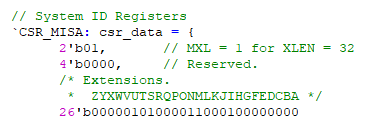
\includegraphics[width=10 cm]{diagrams/misa.png}
                \caption{misa register}
                \label{fig:misa}
        \end{figure}
    
    \item Machine Vendor ID Register mvendorid, Machine Architecture ID Register marchid, Machine Implementation ID Register mimpid & Hart ID Register mhartid\\
        These registers are hardwired to zero.\\

    \item Machine Status Register (mstatus)\\
        The mstatus register keeps track of and controls the hart’s current operating state.
        The main fields in the mstatus registers are shown in fig. \ref{fig:mstatus}
        \begin{figure}[h]
            \centering
            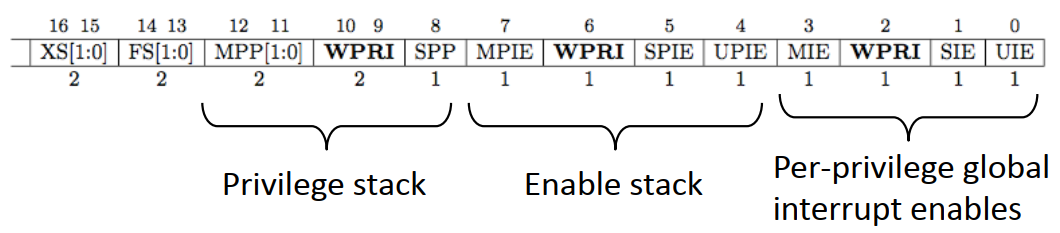
\includegraphics[width=10 cm]{diagrams/mstatus.png}
            \caption{mstatus register}
            \label{fig:mstatus}
        \end{figure}
        Global interrupt-enable bits, MIE, SIE, and UIE, are provided for each privilege mode. When a hart is executing in privilege mode x, interrupts are globally enabled when x IE=1 and globally disabled when x IE=0.\\
        Only take a pending interrupt for privilege mode x if xIE=1 and running in mode x or greater.
        The TSR (Trap SRET) bit supports intercepting the supervisor exception return instruction, SRET. When TSR=1, attempts to execute SRET while executing in S-mode will raise an illegal instruction exception. When TSR=0, this operation is permitted in S-mode.\\
        \begin{figure}[h]
            \centering
            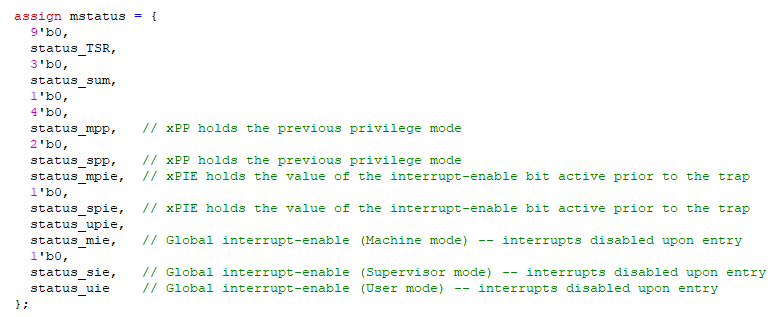
\includegraphics[width=15 cm]{diagrams/mstatus-imp.png}
            \caption{mstatus register implementation}
            \label{fig:mstatus-imp}
        \end{figure}
        Fig. \ref{fig:mstatus-imp} describes the implementation of the mstatus register in our core, the hardwired bits with zero indicates that these functions are not implemented.\\
    
    \item Machine Trap-Vector Base-Address Register (mtvec)\\
        The mtvec register is an MXLEN-bit read/write register that holds trap vector configuration, consisting of a vector base address (BASE) and a vector mode (MODE).
        There are two modes (Direct - Vectored)\\
        When MODE=Direct, all traps into machine mode cause the pc to be set to the address in the BASE field. When MODE=Vectored, all synchronous exceptions into machine mode cause the pc to be set to the address in the BASE field, whereas interrupts cause the pc to be set to the address in the BASE field plus four times the interrupt cause number and we will discuss cause number in mcause register.\\
        In our core we implemented the direct mode.\\
            
    \item Machine Trap Delegation Registers (medeleg and mideleg)\\
        By default, all traps at any privilege level are handled in machine mode, though a machine-mode handler can redirect traps back to the appropriate level with the MRET instruction. The machine exception delegation register (medeleg) and machine interrupt delegation register (mideleg) are 32-bit read/write registers. In systems with S-mode, the medeleg and mideleg registers must exist, and setting a bit in medeleg or mideleg will delegate the corresponding trap, when occurring in S-mode or U-mode, to the Smode trap handler. When a trap is delegated to S-mode, the scause register is written with the trap cause; the sepc register is written with the virtual address of the instruction that took the trap; the stval register is written with an exception-specific datum; the SPP field of mstatus is written with the active privilege mode at the time of the trap; the SPIE field of mstatus is written with the value of the SIE field at the time of the trap; and the SIE field of mstatus is cleared. The mcause, mepc, and mtval registers and the MPP and MPIE fields of mstatus are not written. Traps never transition from a more-privileged mode to a less-privileged mode. For example, if Mmode has delegated illegal instruction exceptions to S-mode, and M-mode software later executes an illegal instruction, the trap is taken in M-mode, rather than being delegated to S-mode. By contrast, traps may be taken horizontally. Using the same example, if M-mode has delegated illegal instruction exceptions to S-mode, and S-mode software later executes an illegal instruction, the trap is taken in S-mode. Delegated interrupts result in the interrupt being masked at the delegator privilege level. For example, if the supervisor timer interrupt (STI) is delegated to S-mode by setting mideleg[5], STIs will not be taken when executing in M-mode. By contrast, if mideleg[5] is clear, STIs can be taken in any mode and regardless of current mode will transfer control to M-mode. medeleg has a bit position allocated for every synchronous exception, with the index of the bit position equal to the value returned in the mcause register (i.e., setting bit 8 allows user-mode environment calls to be delegated to a lower-privilege trap handler). mideleg holds trap delegation bits for individual interrupts, with the layout of bits matching those in the mip register (i.e., STIP interrupt delegation control is located in bit 5). For exceptions that cannot occur in less privileged modes, the corresponding medeleg bits should be hardwired to zero. In particular, medeleg[11] is hardwired to zero.\\
            
    \item Machine Interrupt Registers (mip and mie)\\
        The mip register is an 32-bit read/write register containing information on pending interrupts, while mie is the corresponding 32-bit read/write register containing interrupt enable bits.
        Interrupt cause number i (as reported in CSR mcause) corresponds with bit i in both mip and mie. Bits 15:0 are allocated to standard interrupt causes only, while bits 16 and above are designated for platform or custom use. An interrupt i will be taken if bit i is set in both mip and mie, and if interrupts are globally enabled. By default, M-mode interrupts are globally enabled if the hart’s current privilege mode is less than M, or if the current privilege mode is M and the MIE bit in the mstatus register is set. If bit i in mideleg is set, however, interrupts are considered to be globally enabled if the hart’s current privilege mode equals the delegated privilege mode and that mode’s interrupt enable bit (xIE in mstatus for mode x) is set, or if the current privilege mode is less than the delegated privilege mode. The standard portions (bits 15:0) of registers mip and mie are formatted as shown in Figures \ref{fig:mip} and \ref{fig:mie} respectively.
        \begin{figure}[h]
            \centering
            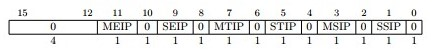
\includegraphics[width=12 cm]{diagrams/mip.jpg}
            \caption{Standard portion (bits 15:0) of mip.}
            \label{fig:mip}
        \end{figure}
            
        \begin{figure}[h]
            \centering
            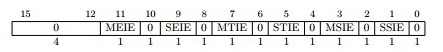
\includegraphics[width=12 cm]{diagrams/mie.jpg}
            \caption{Standard portion (bits 15:0) of mie.}
            \label{fig:mie}
        \end{figure}
        Bits mip.MEIP and mie.MEIE are the interrupt-pending and interrupt-enable bits for machinelevel external interrupts.Bits mip.MTIP and mie.MTIE are the interrupt-pending and interrupt-enable bits for machine timer interrupts. Bits mip.MSIP and mie.MSIE are the interrupt-pending and interrupt-enable bits for machinelevel software interrupts. If supervisor mode is implemented, bits mip.SEIP and mie.SEIE are the interrupt-pending and interrupt-enable bits for supervisor-level external interrupts. SEIP is writable in mip, and may be written by M-mode software to indicate to S-mode that an external interrupt is pending. Additionally, the platform-level interrupt controller may generate supervisor-level external interrupts. Supervisor-level external interrupts are made pending based on the logical-OR of the softwarewritable SEIP bit and the signal from the external interrupt controller. When mip is read with a CSR instruction, the value of the SEIP bit returned in the rd destination register is the logical-OR of the software-writable bit and the interrupt signal from the interrupt controller. However, the value used in the read-modify-write sequence of a CSRRS or CSRRC instruction contains only the software-writable SEIP bit, ignoring the interrupt value from the external interrupt controller. Multiple simultaneous interrupts destined for different privilege modes are handled in decreasing order of destined privilege mode. Multiple simultaneous interrupts destined for the same privilege mode are handled in the following decreasing priority order: MEI, MSI, MTI, SEI, SSI, STI. Synchronous exceptions are of lower priority than all interrupts. Restricted views of the mip and mie registers appear as the sip and sie registers for supervisor level. If an interrupt is delegated to S-mode by setting a bit in the mideleg register, it becomes visible in the sip register and is maskable using the sie register. Otherwise, the corresponding bits in sip and sie appear to be hardwired to zero.\\
        
    \item Machine Scratch Register (mscratch)\\
        The mscratch is an MXLEN-bit read/write register\\
        Typically, it is used to hold a pointer to a machine-mode hart-local context space and swapped with a user register upon entry to an M-mode trap handler.\\
            
    \item Machine Exception Program Counter (mepc)\\
        When a trap is taken into M-mode, mepc is written with the address of the instruction that was interrupted or that encountered the exception. Otherwise, mepc is never written by the implementation, though it may be explicitly written by software.\\
        since our implementation supports only IALIGN=32, the two low bits (mepc[1:0]) are always zero.\\
            
    \item Machine Cause Register (mcause)\\
        When a trap is taken into M-mode, mcause is written with a code indicating the event that caused the trap. Otherwise, mcause is never written by the implementation, though it may be explicitly written by software.\\
        \begin{figure}[h]
            \centering
            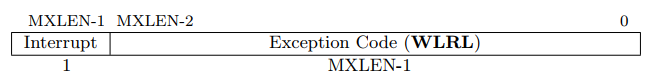
\includegraphics[width=10 cm]{diagrams/mcause.png}
            \caption{mcause register}
            \label{fig:mcause}
        \end{figure}
        As shown in fig. \ref{fig:mcause}, the Interrupt bit in the mcause register is set if the trap was caused by an interrupt. The Exception Code field contains a code identifying the last exception. fig. \ref{fig:exception-code} lists the possible machine-level exception codes.\\
        \begin{figure}[h!]
            \centering
            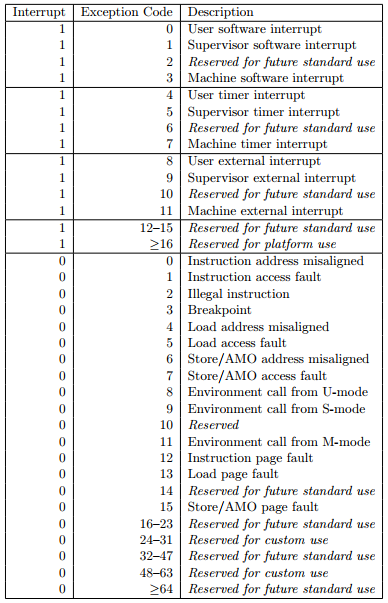
\includegraphics[width=10 cm]{diagrams/exception_code.png}
            \caption{exception codes}
            \label{fig:exception-code}
        \end{figure}
        
    \item Machine Trap Value (mtval) Register\\
       	   When a trap is taken into M-mode, mtval is either set to zero or written with exception-specific information to assist software in handling the trap. Otherwise, mtval is never written by the implementation, though it may be explicitly written by software. The hardware platform will specify which exceptions must set mtval informatively and which may unconditionally set it to zero.
		    \item  Machine Time (mtime and mtimecmp) Registers\\
            Platforms provide a real-time counter, exposed as a memory-mapped machine-mode register
            \begin{figure}[h]
            \centering
            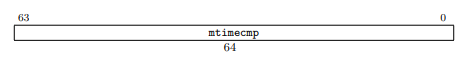
\includegraphics[width=10 cm]{diagrams/mtimecmp.PNG}
            \caption{mtimecmp register}
            \label{fig:mtimecmp}
            \end{figure}As shown in fig. \ref{fig:mtimecmp}
            , mtime 
            \begin{figure}[h]
            \centering
            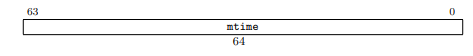
\includegraphics[width=10 cm]{diagrams/mtime.PNG}
            \caption{mtime register}
            \label{fig:mtime}
            \end{figure}As shown in fig. \ref{fig:mtime}.
mtime must run at constant frequency, and the platform must provide a mechanism for determining
the timebase of mtime.
The mtime register has a 64-bit precision on all RV32, RV64, and RV128 systems.
Platforms provide
a 64-bit memory-mapped machine-mode timer compare register (mtimecmp), which causes a timer
interrupt to be posted when the mtime register contains a value greater than or equal to the value

in the mtimecmp register. The interrupt remains posted until it is cleared by writing the mtimecmp
register. The interrupt will only be taken if interrupts are enabled and the MTIE bit is set in the
mie register\\
\\

            
            
            
          
 \item Machine Performance Counter (mcycle(h)) Register \\
 M-mode includes a basic hardware performance monitoring facility.The mcycle CSR holds a count of the number of cycles the hart has executed since some arbitrary time in the past. 
 \begin{figure}[h]
            \centering
            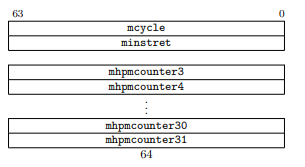
\includegraphics[width=10 cm]{diagrams/mcycle.PNG}
            \caption{mcycle register}
            \label{fig:mcycle}
            \end{figure}As shown in fig. \ref{fig:mcycle}
            
 The mcycle register has 64-bit precision on all RV32, RV64, and RV128 systems.
On RV32 only, reads of the mcycle, minstret, and mhpmcountern CSRs return the low 32 bits, while reads of the mcycleh, minstreth, and mhpmcounternh CSRs return bits 63–32 of the corresponding
counter\\
\\
\begin{figure}[h]
    \centering
  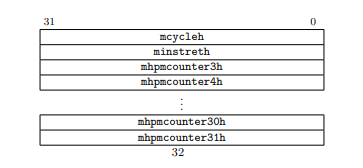
\includegraphics[width=10 cm]{diagrams/mcycleh.PNG}
 \caption{mcycleh register}
 \label{fig:mcycleh}
     \end{figure}As shown in fig. \ref{fig:mcycleh}
\end{itemize}
%%%%%%%%%%%%%%%%%%%%%%%%%%%%%%%%%%%%%%%%%%%%%%%%%%%%%%%%%%%%%%%%%
\subsection{Supervisor-Level ISA}
This section describes the supervisor-level operations available in supervisor-mode (S-mode),which is two layers below Machine mode, as shown in table \ref{table:modes}, S-mode code can access CSRs at user-level, but it can not access CSRs at machine-level.An operating system runs at S-mode.

\subsubsection{Supervisor-Level CSRs}
Supervisor-mode has a similar number of CSRs as in machine-mode, though most of them are subsets of their equivalent machine-mode CSRs.

\begin{itemize}
    \item Supervisor Status Register sstatus\\
        The sstatus register keeps track of the processor’s current operating state.The main fields in the sstatus register are shown in fig. \ref{fig:sstatus}
        \begin{figure}[h]
            \centering
            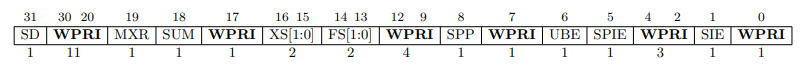
\includegraphics[width=10 cm]{diagrams/sstatus.png}
            \caption{sstatus register}
            \label{fig:sstatus}
        \end{figure}
        The SIE bit is the interrupt enable bit in supervisor mode. supervisor mode interrupts are globally enabled When SIE = 1 and globally disabled when SIE = 0. When the hart is running in user-mode, the value in SIE is ignored, and supervisor-level interrupts are enabled.\\
        The SPP bit indicates the privilege level at which a hart was executing before entering supervisor mode. When a trap is taken, SPP is set to 0 if the trap originated from user mode, or 1 otherwise.\\
        The SPIE bit indicates whether supervisor interrupts were enabled prior to trapping into supervisor mode. When a trap is taken into supervisor mode, SPIE is set to SIE, and SIE is set to 0.\\ figure \ref{fig:sstatus_imp}  describes the implementation of the sstatus register in our core.
        
        \begin{figure}[h]
            \centering
            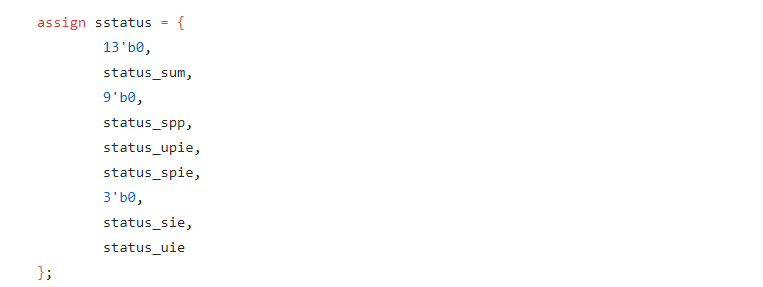
\includegraphics[width=15 cm]{diagrams/sstatus_imp.png}
            \caption{sstatus register  implementation}
            \label{fig:sstatus_imp}
        \end{figure} \\
        
        Hardwired bits with zero indicates that these functions are not implemented.
         
    \item Supervisor Trap Vector Base Address Register stvec \\
        The stvec register is an SXLEN-bit read/write register that holds trap vector configuration, consisting of a vector base address (BASE) and a vector mode (MODE).There are two modes (Direct - Vectored).\\ 
        When MODE=Direct, all traps into  supervisor mode cause the pc to be set to the address in the BASE field. When MODE=Vectored, all synchronous exceptions into supervisor mode cause the pc to be set to the address in the BASE field, whereas interrupts cause the pc to be set to the address in the BASE field plus four times the interrupt cause number.\\
        In our core we implemented the direct mode.
          
    \item Supervisor Interrupt Registers sip and sie\\
        The sip register is a 32-bit read/write containing information on pending interrupts,while sie is a 32-bit read/write containing interrupt enable bits. Interrupt cause number i (as reported in CSR scause) corresponds with bit i in both sip and sie. Bits 15:0 are allocated to standard interrupt causes only, while bits 16 and above are designated for platform or custom use.\\
        An interrupt will be taken if the corresponding bits is set in both sie and sip, and if supervisor-level interrupts are globally enabled if the hart’s current privilege mode is less than S, or if the current privilege mode is S and the SIE bit in the sstatus register is set. The standard portions (bits 15:0) of registers mip and mie are formatted as shown in Figures \ref{fig:sip} and \ref{fig:sie} respectively.
        
        \begin{figure}[h]
            \centering
            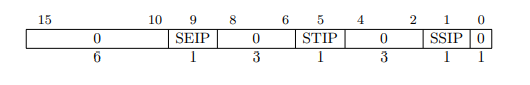
\includegraphics[width=12 cm]{diagrams/sip.PNG}
            \caption{Standard portion (bits 15:0) of sip.}
            \label{fig:sip}
        \end{figure}
            
        \begin{figure}[h]
            \centering
            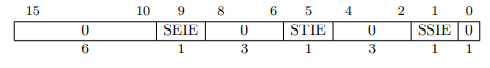
\includegraphics[width=12 cm]{diagrams/sie.PNG}
            \caption{Standard portion (bits 15:0) of sie.}
            \label{fig:sie}
        \end{figure}
            
        Bits sip.SEIP and sie.SEIE are the interrupt-pending and interrupt-enable bits for supervisor level external interrupts.
        Bits sip.STIP and sie.STIE are the interrupt-pending and interrupt-enable bits for supervisor timer interrupts.
        Bits sip.SSIP and sie.SSIE are the interrupt-pending and interrupt-enable bits for supervisor level software interrupts.
          
    \item Supervisor Trap Delegation Registers sedeleg and sideleg \\
        For systems with both S-mode and the U-mode, CSRs sedeleg and sideleg are added. These registers have the same layout as the machine trap delegation registers, medeleg and mideleg. sedeleg and sideleg allow S-mode to delegate traps to U-mode. Only bits corresponding to traps that have been delegated to S-mode are writable; the others are hardwired to zero. Setting a bit in sedeleg or sideleg delegates the corresponding trap in U-mode to the U-mode trap handler.

    \item Supervisor Scratch Register sscratch \\
        The sscratch register is an SXLEN-bit read/write register, dedicated for use by the supervisor. Typically, sscratch is used to hold a pointer to the hart-local supervisor context while the hart is executing user code. At the beginning of a trap handler, sscratch is swapped with a user register to provide an initial working register.
          
    \item  Supervisor Exception Program Counter sepc \\
        When a trap is taken into S-mode, sepc is written with the address of the instruction that was interrupted or that encountered the exception. Otherwise, sepc is never written by the implementation, though it may be explicitly written by software.\\
        Since our implementation supports only IALIGN=32, the two low bits (sepc[1:0]) are always zero.\\
          
    \item Supervisor Cause Register scause \\
        When a trap is taken into S-mode, scause is written with a code indicating the event that caused the trap. Otherwise, scause is never written by the implementation, though it may be explicitly written by software.\\
        
        \begin{figure}[h]
            \centering
            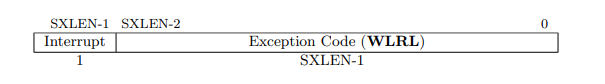
\includegraphics[width=10 cm]{diagrams/scause.png}
            \caption{scause register}
            \label{fig:scause}
        \end{figure}As shown in fig. \ref{fig:scause}
        
        The Interrupt bit in the scause register is set if the trap was caused by an interrupt. The Exception Code field contains a code identifying the last exception. Figure \ref{fig:exception-code} lists the possible exception codes.\\
          
    \item Supervisor Trap Value (stval) Register \\
        When a trap is taken into S-mode, stval is either set to zero or written with exception-specific information to assist software in handling the trap. Otherwise, stval is never written by the implementation, though it may be explicitly written by software. The hardware platform will specify which exceptions must set stval informatively and which may unconditionally set it to zero.
\end{itemize}


%%%%%%%%%%%%%%%%%%%%%%%%%%%%%%%%%%%%%%%%%%%%%%%%%%%%%%%%%%%%%%%%%
\subsection{“N” Standard Extension for User-Level Interrupts}
When the N extension is present, and the outer execution environment has delegated designated
interrupts and exceptions to user-level, then hardware can transfer control directly to a user-level
trap handler without invoking the outer execution environment.

\subsubsection{Additional CSRs}
New user-visible CSRs are added to support the N extension.
\begin{itemize}
    \item User Status Register (ustatus)\\
        The ustatus register is a 32-bit read/write register formatted as shown in Figure \ref{fig:ustatus}. The ustatus register keeps track of and controls the hart’s current operating state.
        
        \begin{figure}[h!]
            \centering
            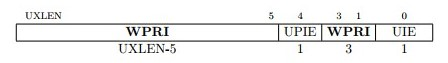
\includegraphics[width=10 cm]{diagrams/ustatus.jpg}
            \caption{User-mode status register (ustatus).}
            \label{fig:ustatus}
        \end{figure}

        The user interrupt-enable bit UIE disables user-level interrupts when clear. The value of UIE is copied into UPIE when a user-level trap is taken, and the value of UIE is set to zero to provide atomicity for the user-level trap handler. The UIE and UPIE bits are mirrored in the mstatus and sstatus registers in the same bit positions.\\

    \item User Interrupt Registers (uip and uie)\\
        The uip register is a UXLEN-bit read/write register containing information on pending interrupts, while uie is the corresponding UXLEN-bit read/write register containing interrupt enable bits.
        \begin{figure}[h!]
            \centering
            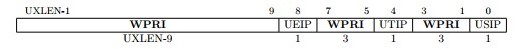
\includegraphics[width=15 cm]{diagrams/uip.jpg}
            \caption{User interrupt-pending register (uip).}
            \label{fig:uip}
        \end{figure}

        \begin{figure}[h!]
            \centering
            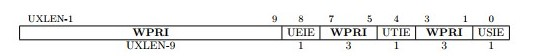
\includegraphics[width=15 cm]{diagrams/uie.jpg}
            \caption{User interrupt-enable register (uie)}
            \label{fig:uie}
        \end{figure}

        Three types of interrupts are defined: software interrupts, timer interrupts, and external interrupts. A user-level software interrupt is triggered on the current hart by writing 1 to its user software interrupt-pending (USIP) bit in the uip register. A pending user-level software interrupt can be cleared by writing 0 to the USIP bit in uip. User-level software interrupts are disabled when the USIE bit in the uie register is clear. The ABI should provide a mechanism to send interprocessor interrupts to other harts, which will ultimately cause the USIP bit to be set in the recipient hart’s uip register. All bits besides USIP in the uip register are read-only.
        
        A user-level timer interrupt is pending if the UTIP bit in the uip register is set. User-level timer interrupts are disabled when the UTIE bit in the uie register is clear. The ABI should provide a mechanism to clear a pending timer interrupt. A user-level external interrupt is pending if the UEIP bit in the uip register is set. User-level external interrupts are disabled when the UEIE bit in the uie register is clear. The ABI should provide facilities to mask, unmask, and query the cause of external interrupts.
        
        The uip and uie registers are subsets of the mip and mie registers. Reading any field, or writing any writable field, of uip/uie effects a read or write of the homonymous field of mip/mie. If S-mode is implemented, the uip and uie registers are also subsets of the sip and sie registers.\\

    \item Supervisor Trap Delegation Registers (sedeleg and sideleg)\\
        For systems with both S-mode and the N extension, new CSRs sedeleg and sideleg are added. These registers have the same layout as the machine trap delegation registers, medeleg and mideleg. sedeleg and sideleg allow S-mode to delegate traps to U-mode. Only bits corresponding to traps that have been delegated to S-mode are writable; the others are hardwired to zero. Setting a bit in sedeleg or sideleg delegates the corresponding trap in U-mode to the U-mode trap handler.\\

    \item Other CSRs\\
        The uscratch, uepc, ucause, utvec, and utval CSRs are defined analogously to the mscratch, mepc, mcause, mtvec, and mtval CSRs.\\
\end{itemize}
%%%%%%%%%%%%%%%%%%%%%%%%%%%%%%%%%%%%%%%%%%%%%%%%%%%%%%%%%%%%%%%%
\subsubsection{Privileged Instructions}

\begin{itemize}
    \item Environment Call\\
        The ECALL instruction shown in fig. \ref{fig:ecall} is used to make a request to the supporting execution environment. When executed in U-mode, S-mode, or M-mode, it generates an environment-call-from-U-mode exception, environment-call-from-S-mode exception, or environment-call-from-M-mode exception, respectively, and performs no other operation.\\
        \begin{figure}[h!]
            \centering
            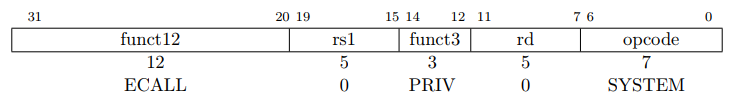
\includegraphics[width=10 cm]{diagrams/ecall.png}
            \caption{ECALL Instruction}
            \label{fig:ecall}
        \end{figure}
            
    \item Trap-Return Instructions\\
        To return after handling a trap, there are separate trap return instructions per privilege level: MRET, SRET, and URET shown in fig. \ref{fig:ret}.\\
        \begin{figure}[h!]
            \centering
            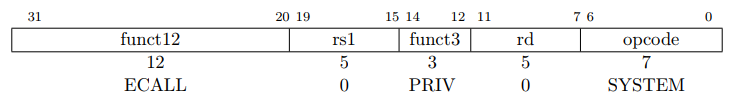
\includegraphics[width=10 cm]{diagrams/ecall.png}
            \caption{Return Instructions}
            \label{fig:ret}
        \end{figure}
        An xRET instruction can be executed in privilege mode x or higher, where executing a lower-privilege xRET instruction will pop the relevant lower-privilege interrupt enable and privilege mode stack. In addition to manipulating the privilege stack, xRET sets the pc to the value stored in the xepc register.
\end{itemize}

Upon reset, a hart’s privilege mode is set to M. The mstatus fields MIE and MPRV are reset to 0.


%%%%%%%%%%%%%%%%%%%%%%%%%%%%%%%%%%%%%%%%%%%%%%%%%%%%%%%%%%%%%%%%%
    
%%%%%%%%%%%%%%%%%%%%%%%%%%%%%%%%%%%%%%%%%%%%%%%%%%%%%%%%%%%%%%%%%
\section{Interrupt Controller}
RISC-V defines the following interrupts per Hart:
\begin{itemize}
    \item Software – architecturally defined software interrupt
    \item Timer – architecturally defined timer interrupt
    \item External – Peripheral Interrupts
\end{itemize}
\textbf{Core Local Interrupter (CLINT)}\\
The CLINT has a fixed priority scheme which implements Software, Timer, and External interrupts. Software preemption is only available between privilege levels using the CLINT. For example, while in Supervisor mode, a Machine mode interrupt will immediately take priority and preempt Supervisor mode operation. Preemption within a privilege level is not supported with the CLINT. The interrupt ID represents the fixed priority value of each interrupt, and is not configurable. There are two different CLINT modes of operation, direct mode and vectored mode. To configure CLINT modes, write mtvec.mode field, which is bit[0] of mtvec CSR. For direct mode, mtvec.mode=0, and for vectored mode mtvec.mode=1. Direct mode is the default reset value. The mtvec.base holds the base address for interrupts and exceptions, and must be a minimum 4-byte aligned value in direct mode.\\
In our design we used the direct mode, Direct mode means all interrupts and exceptions trap to the same handler, and there is no vector table implemented. It is software’s responsibility to execute code to figure out which interrupt occurred. The software handler in direct mode should first read mcause.interrupt to determine if an interrupt or exception occurred, then decide what to do based on mcause.code value which contains the respective interrupt or exception code.\\
\newline
\noindent The trap handler - entry and exit are performed as the following:
\begin{enumerate}
    \item Save \textbf{\textit{pc}} to \textbf{\textit{mepc}}.
    \item Save Privilege level to \textbf{\textit{mstatus.mpp}}.
    \item Save \textbf{\textit{mie}} to \textbf{\textit{mstatus.mpie}}.
    \item Set \textbf{\textit{pc}} to interrupt handler address, based on mode of operation.
    \item Disable interrupts by setting \textbf{\textit{mstatus.mie=0}}\\
    \textit{At this point control is handed over to software where the interrupt processing begins. At the end of the interrupt handler, the mret instruction will do the following.}
    \item Restore \textbf{\textit{mepc}} to \textbf{\textit{pc}}.
    \item Restore Privilege level to \textbf{\textit{mstatus.mpp}}.
    \item Restore \textbf{\textit{mstatus.mpie}} to \textbf{\textit{mie}}.
\end{enumerate}
\end{document}